%%%%%%%%%%%%%%%%
\section{Outer Controller}

\begin{frame}{Outer Controller}{Path Generation Algorithm}
    \begin{figure}[H]
        \centering
        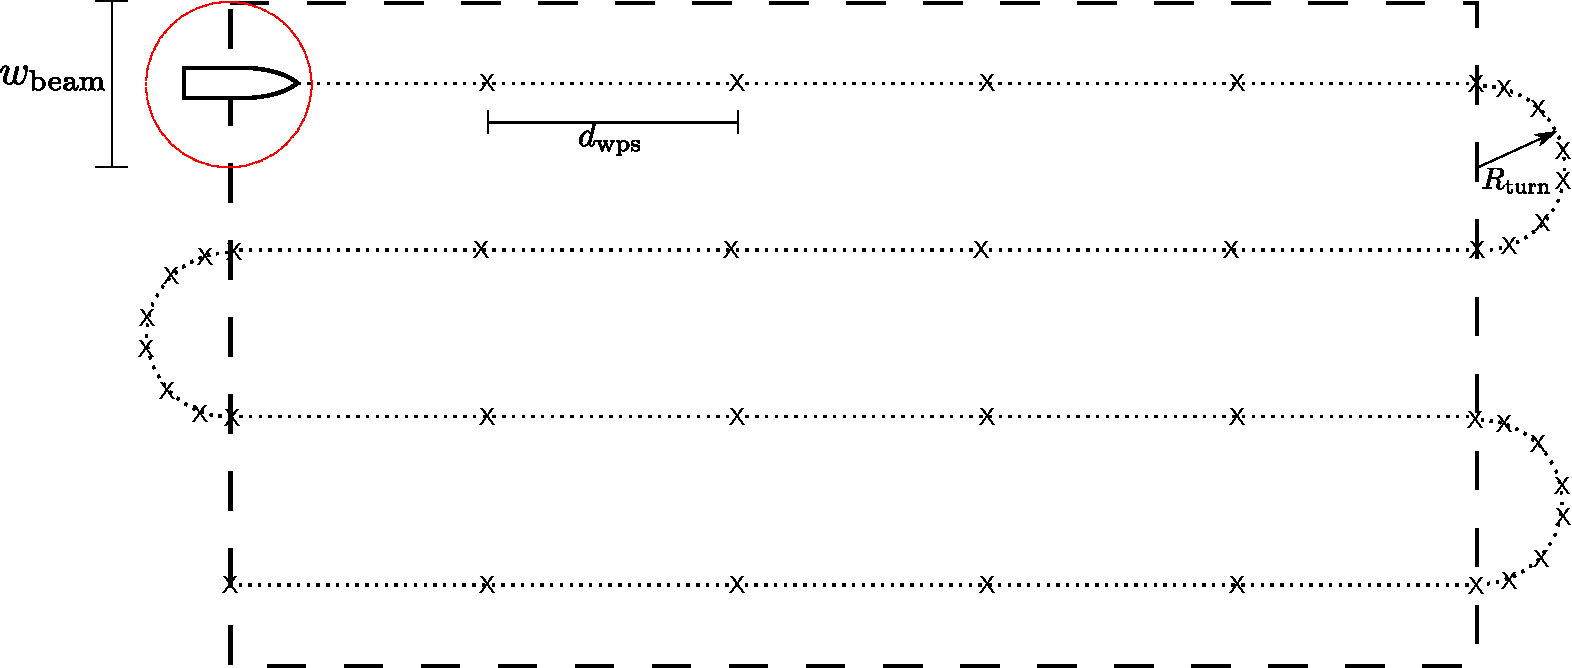
\includegraphics[width=1\textwidth]{figures/pathGen} 
    \end{figure}       
\end{frame}

\begin{frame}{Outer Controller}{Path Following Algorithm}
    \begin{minipage}{0.6\linewidth}
        \uncover<1-4>{
        \begin{figure}[H]
            \centering
            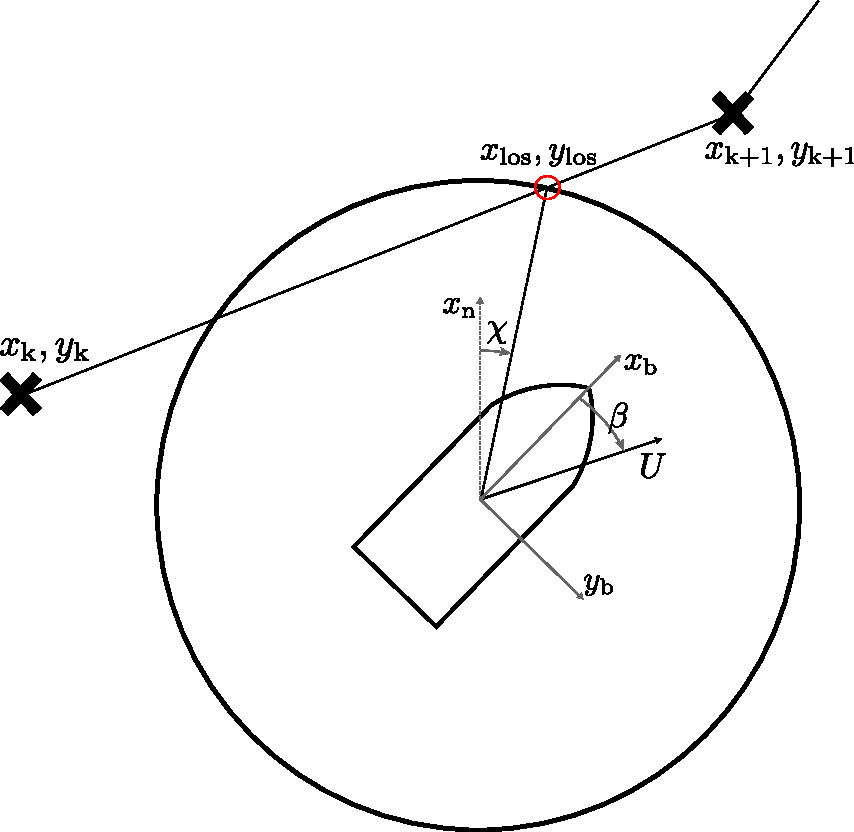
\includegraphics[width=0.9\linewidth]{figures/LOSalgorithm}
        \end{figure} }       
    \end{minipage}\hfill      
    \begin{minipage}{0.2\linewidth}
        \uncover<2-4>{
        \begin{flalign}
            \chi &= \arctan\left(\frac{y_\mathrm{LOS}-y_\mathrm{n}}{x_\mathrm{LOS}-x_\mathrm{n}}\right)\nonumber 
        \end{flalign} }
        \uncover<3-4>{
        \begin{flalign}
            \beta &= \arctan\left(\frac{\dot{y}_\mathrm{b}}{\dot{x}_\mathrm{b}}\right) \nonumber
        \end{flalign} }
        \uncover<4>{
        \begin{flalign}
            \psi&_\mathrm{ref} = \chi - \beta \nonumber
        \end{flalign}}          
    \end{minipage}\hfill \\ 
\end{frame}

\begin{frame}{Outer Controller}{Path Following Algorithm}
    \begin{itemize}
        \item Change active waypoints
    \end{itemize}
    \begin{figure}[H]
        \centering
        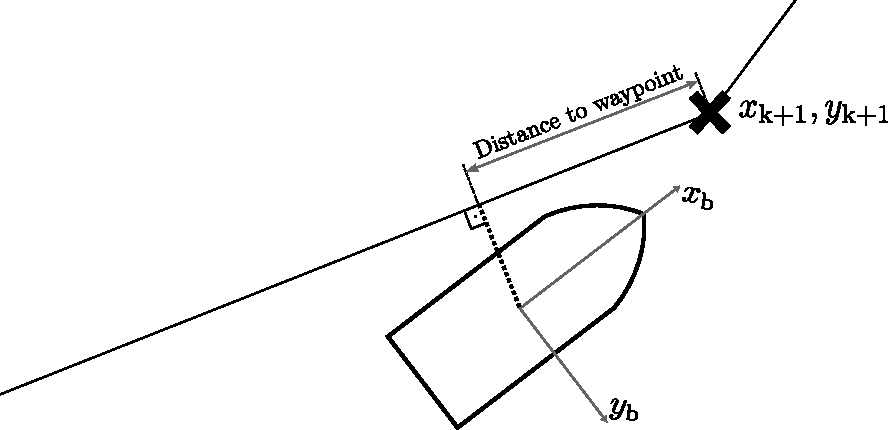
\includegraphics[width=0.6\linewidth]{figures/LOSalgorithmdistancewp}
    \end{figure}
\end{frame}
\begin{frame}{Outer Controller}{Path Following Algorithm}
    \begin{itemize}
        \item Convergence to the path
    \end{itemize}
    \begin{minipage}{0.45\linewidth}
        \begin{figure}[H]
            \centering
            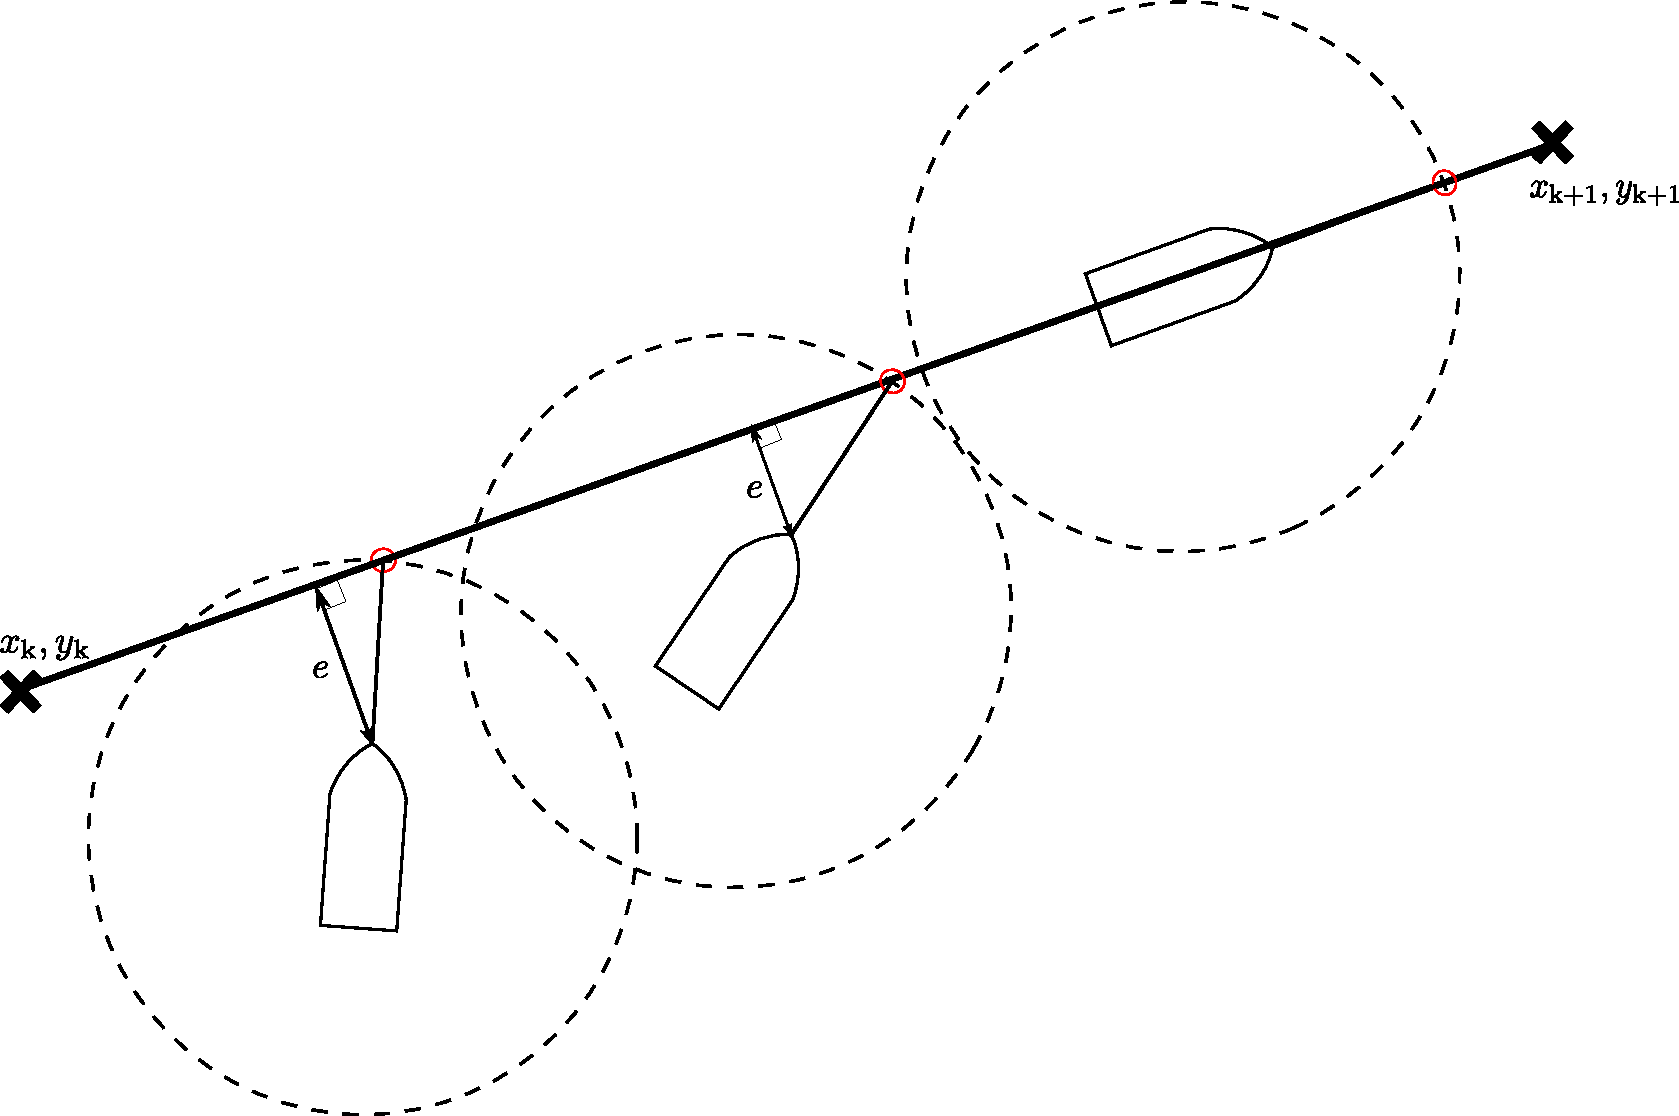
\includegraphics[width=1\linewidth]{figures/patherror}
        \end{figure}     
    \end{minipage}\hfill      
    \begin{minipage}{0.45\linewidth}
        \begin{figure}[H]
            \centering
            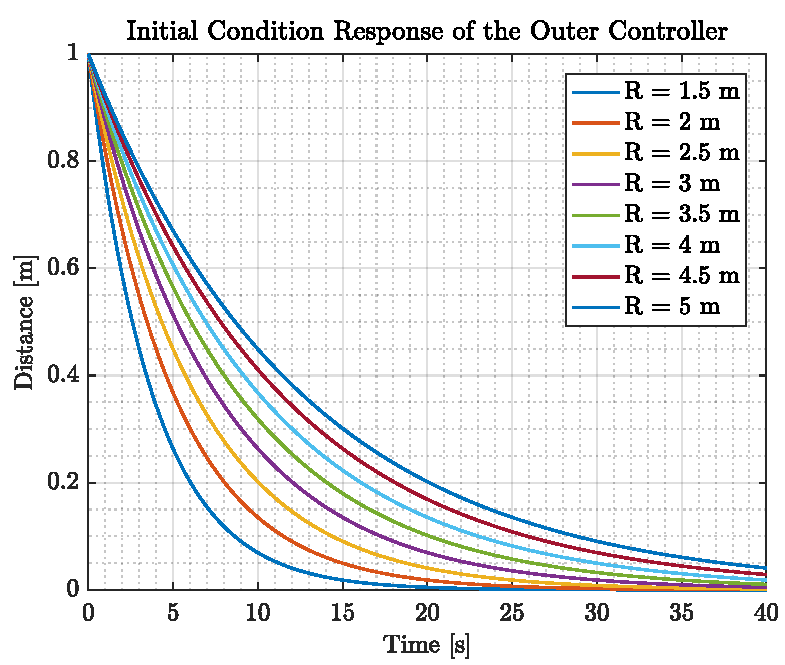
\includegraphics[width=1\linewidth]{figures/initCondOuter}
        \end{figure}               
    \end{minipage}\hfill \\
\end{frame}
%%%%%%%%%%%%%%%%
\section{Results}

\begin{frame}{Results}{Controller Results}
\begin{itemize}
    \item LQR as inner controller
\end{itemize}
    \begin{minipage}{0.45\linewidth}
            \begin{figure}[H]
                \centering
                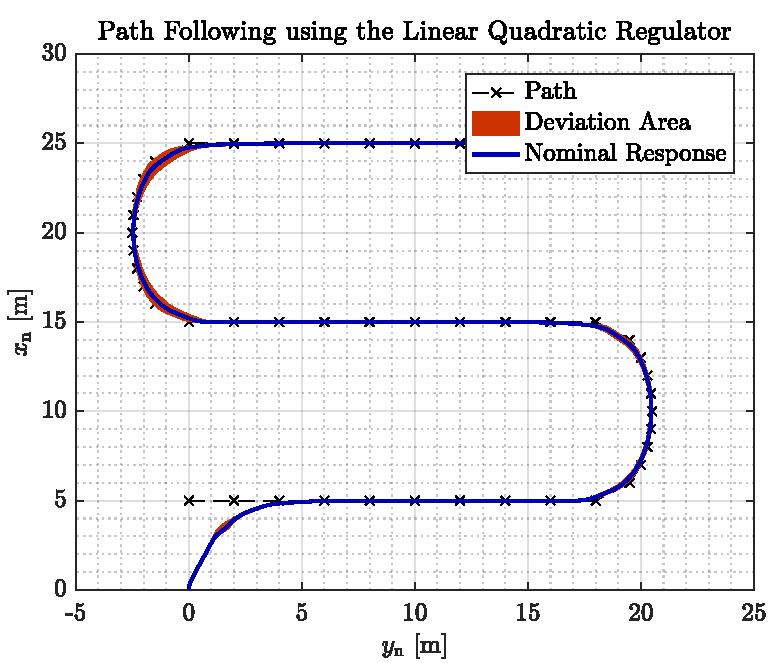
\includegraphics[width=1\linewidth]{figures/path_lqr}
            \end{figure}        
        \end{minipage}\hfill      
    \begin{minipage}{0.45\linewidth}
            \begin{figure}[H]
                \centering
                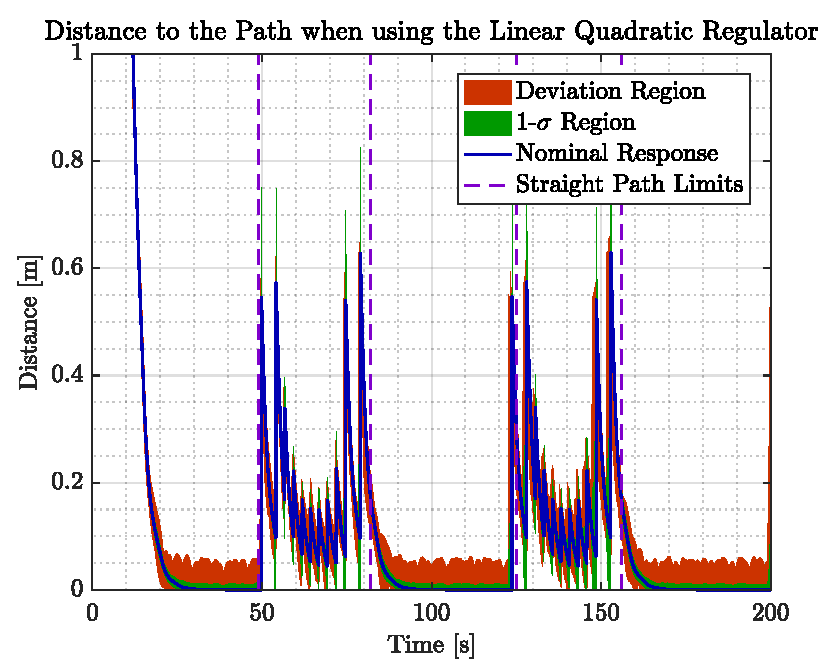
\includegraphics[width=1\linewidth]{figures/dist_lqr}
            \end{figure}               
        \end{minipage}\hfill \\    
\end{frame}

\begin{frame}{Results}{Controller Results}
    \begin{itemize}
        \item Robust controller as inner controller
    \end{itemize}
    \begin{minipage}{0.45\linewidth}
            \begin{figure}[H]
                \centering
                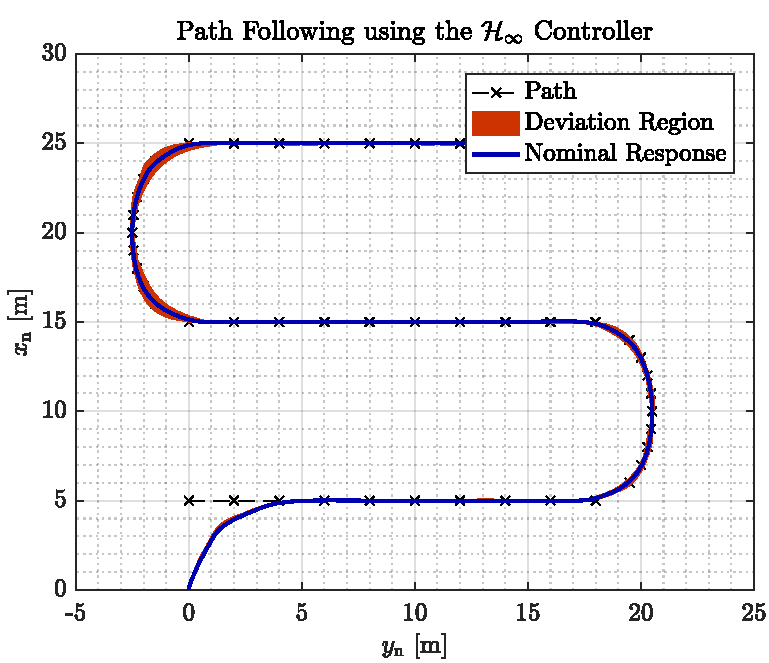
\includegraphics[width=1\linewidth]{figures/path_rob}
            \end{figure}       
        \end{minipage}\hfill      
    \begin{minipage}{0.45\linewidth}
            \begin{figure}[H]
                \centering
                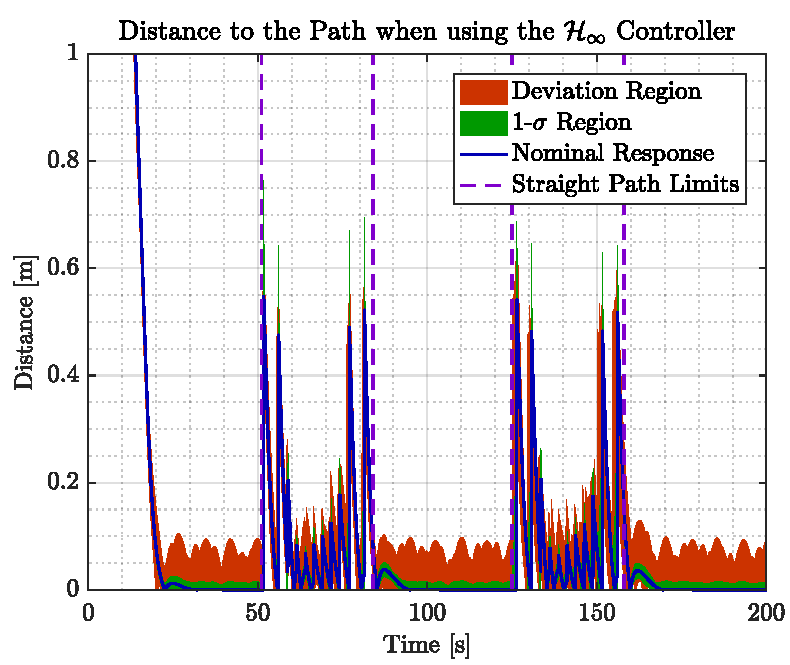
\includegraphics[width=1\linewidth]{figures/dist_rob}
            \end{figure}             
        \end{minipage}\hfill \\    
\end{frame}

%\begin{frame}{Results}{Implementation Results}
%    \begin{itemize}
%        \item Implementation diagram in ROS
%    \end{itemize}
%    \begin{figure}[H]
%        \centering
%        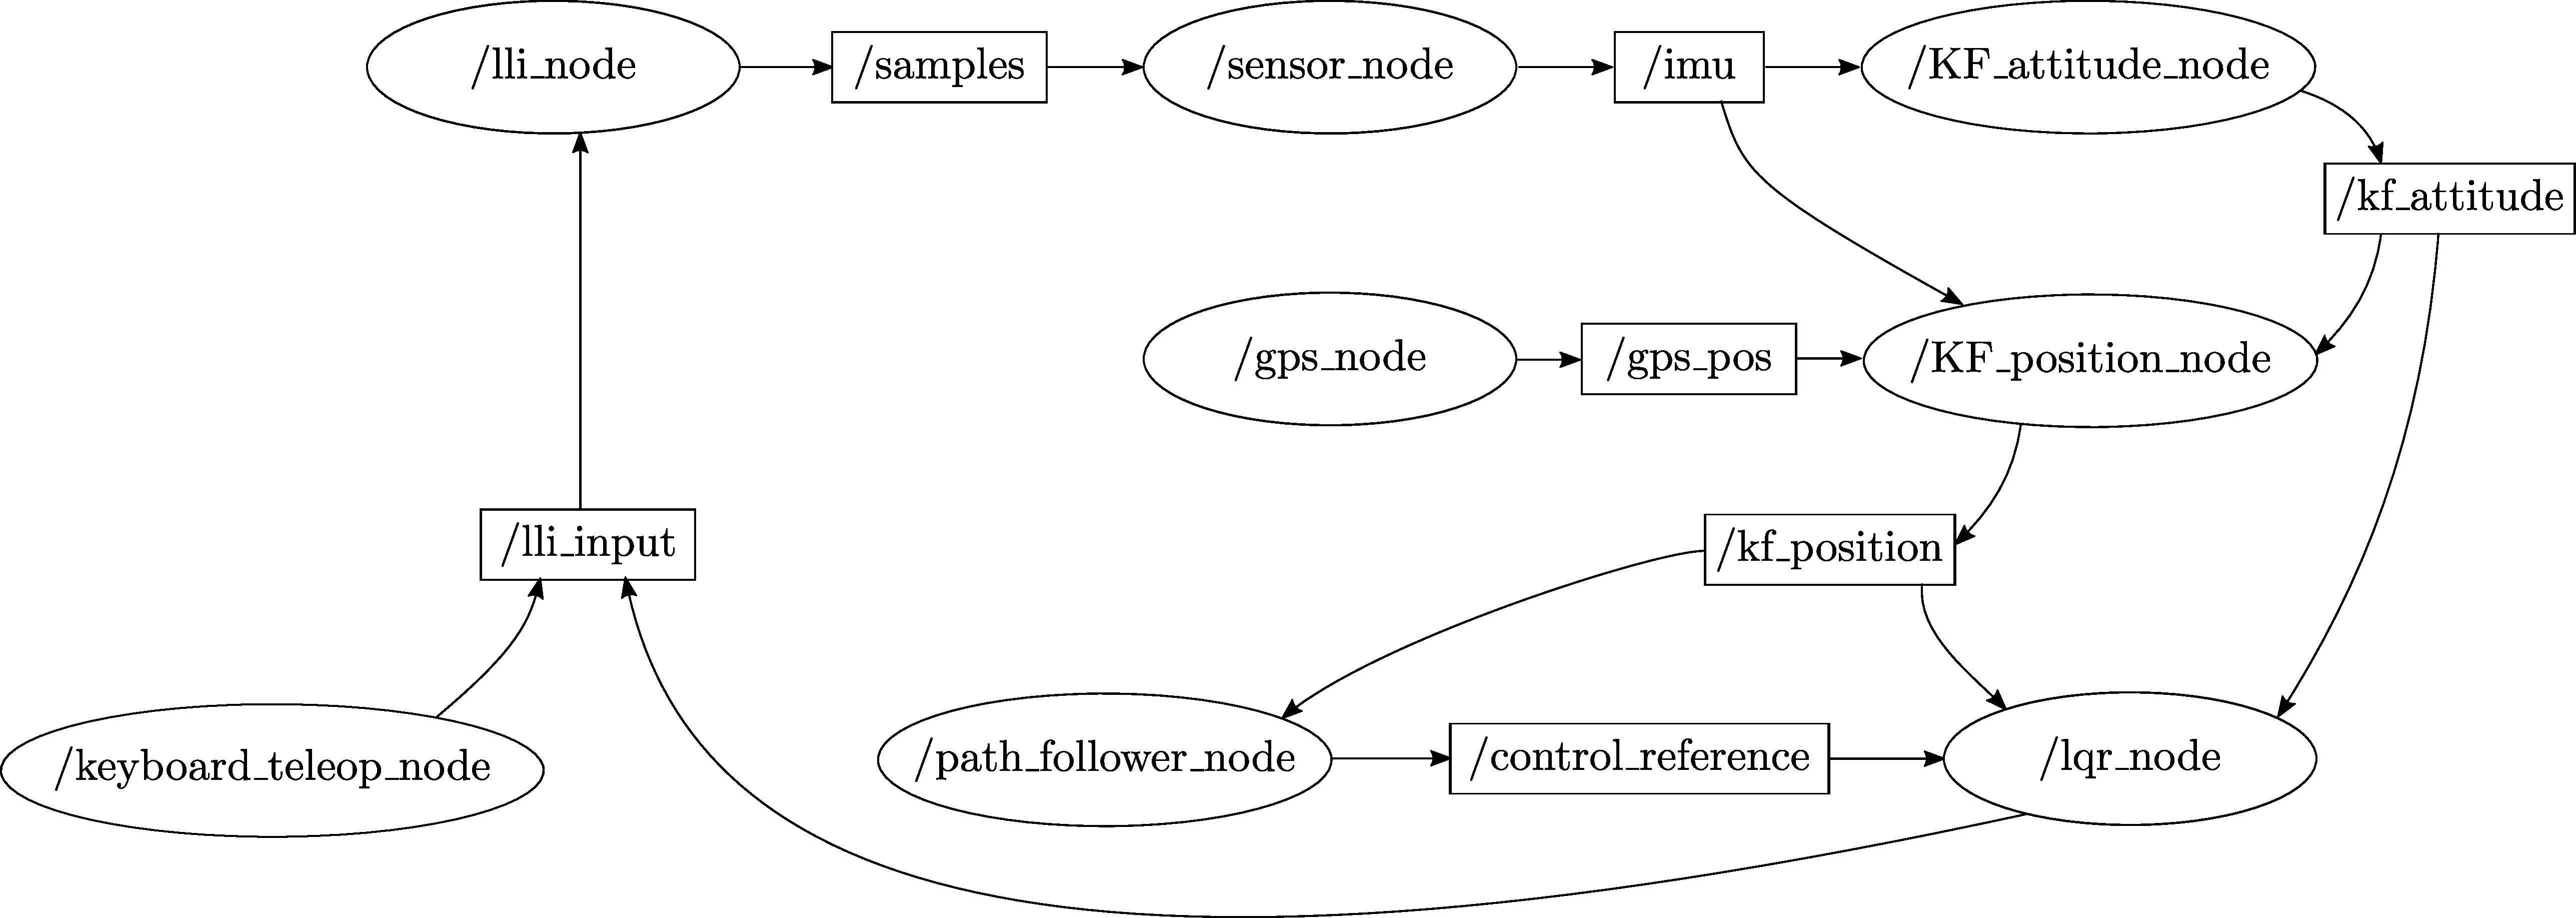
\includegraphics[width=1\textwidth]{figures/diagramROS}
%    \end{figure}  
%\end{frame}


\begin{frame}{Results}{Implementation Results}
    \begin{itemize}
        \item Inner controller test
    \end{itemize}
    \begin{minipage}{0.45\linewidth}
        \begin{figure}[H]
            \centering
            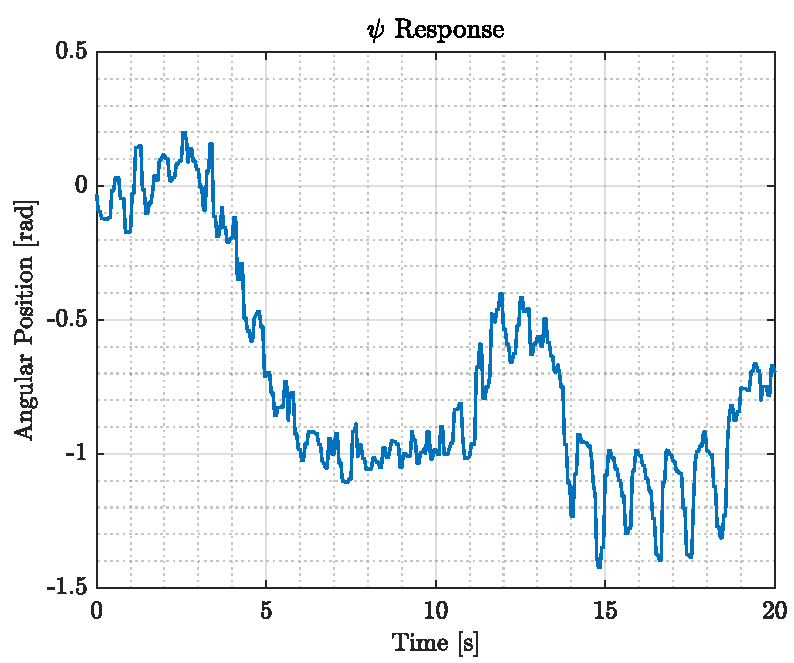
\includegraphics[width=1\linewidth]{figures/inner_yaw}
        \end{figure}       
    \end{minipage}\hfill      
    \begin{minipage}{0.45\linewidth}
        \begin{figure}[H]
            \centering
            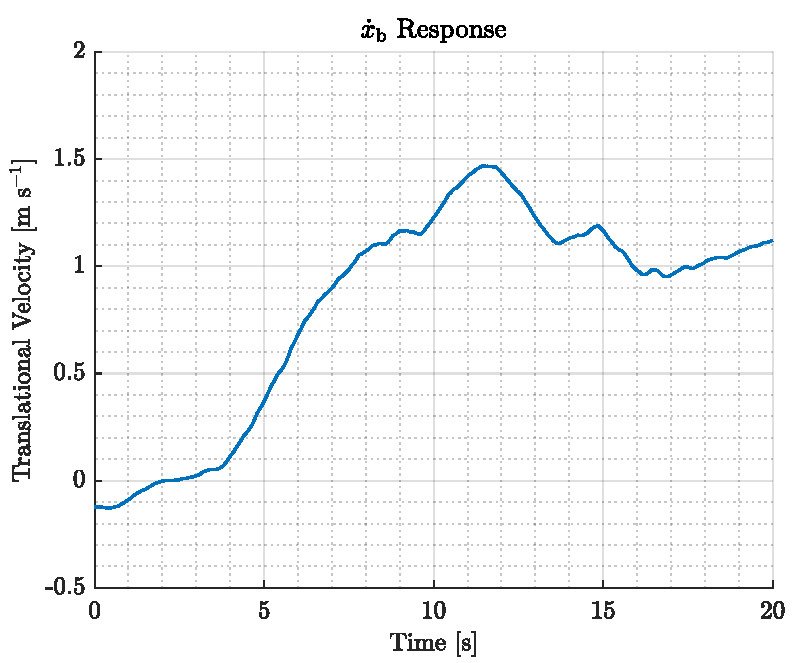
\includegraphics[width=1\linewidth]{figures/inner_xbdot}
        \end{figure}             
    \end{minipage}\hfill \\    
\end{frame}

\begin{frame}{Results}{Implementation Results}
    \begin{itemize}
        \item Actuator tests
    \end{itemize}
    \begin{minipage}{0.45\linewidth}
        \begin{figure}[H]
            \centering
            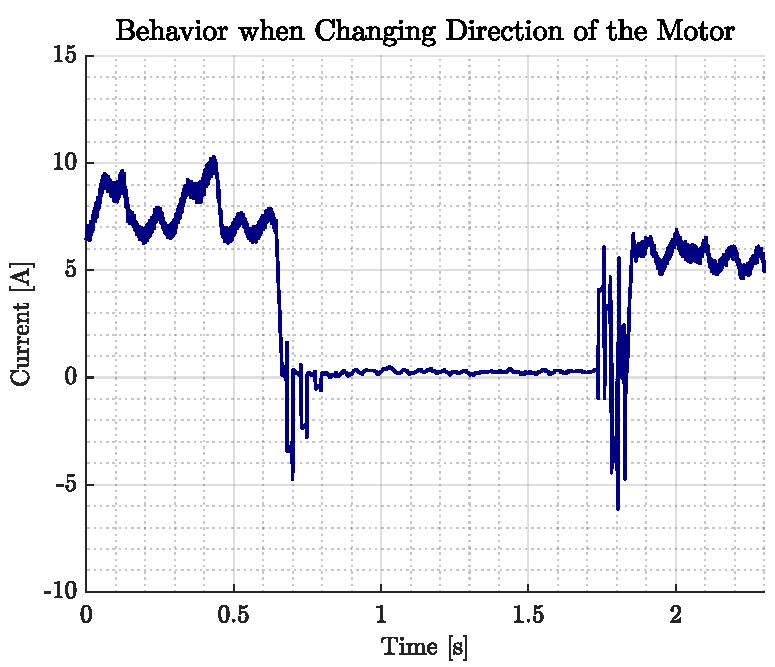
\includegraphics[width=1\linewidth]{figures/direction}
        \end{figure}       
    \end{minipage}\hfill      
    \begin{minipage}{0.45\linewidth}
        \begin{figure}[H]
            \centering
            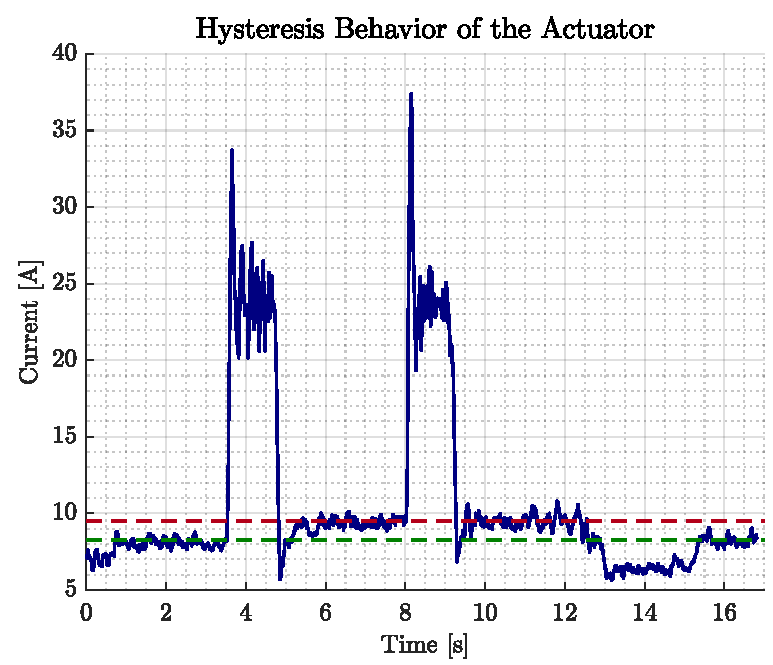
\includegraphics[width=1\linewidth]{figures/hysteresis}
        \end{figure}             
    \end{minipage}\hfill \\    
\end{frame}

%%%%%%%%%%%%%%%%
\section{Conclusion}

\begin{frame}{Conclusion}{}
    \begin{itemize}
        \item A dynamic model of the system has been derived
    \end{itemize}
    \begin{itemize}
        \item The estimator has been designed and tested through simulation
    \end{itemize}
    \begin{itemize}
        \item The control system has also been analyzed through simulations that include disturbances, noise and varying parameters
    \end{itemize}
    \begin{itemize}
        \item The simulated results have not been fully replicated in the real vessel, but they show a promising behavior of the control system
    \end{itemize}
\end{frame}